\documentclass[a4paper,12pt]{article}

\usepackage[utf8]{inputenc}
\usepackage[T1]{fontenc}
\usepackage{textcomp}
\usepackage{amssymb}
\usepackage[czech]{babel}
\usepackage{geometry}
\usepackage{hyperref}
\usepackage{booktabs}
\usepackage{longtable}
\usepackage{array}
\usepackage{enumitem}
\usepackage{xcolor}
\usepackage{titlesec}
\usepackage{parskip}
\usepackage{microtype}
\usepackage{fancyhdr}
\usepackage{etoolbox}
\usepackage{graphicx}
\usepackage{rotating}

\geometry{margin=2.5cm}

\hypersetup{
  colorlinks=true,
  linkcolor=black,
  urlcolor=blue,
}

\pagestyle{fancy}
\fancyhf{}
\rhead{KIV/UUR — Semestrální práce}
\lhead{CampMaster 3000}
\rfoot{\thepage}

% Číslované sekce, každá hlavní sekce začíná na nové stránce
\titleformat{\section}{\large\bfseries}{\thesection.}{0.6em}{}[\titlerule]
\titleformat{\subsection}{\normalsize\bfseries}{\thesubsection}{0.5em}{}

\preto\section{\clearpage}

\definecolor{okgreen}{rgb}{0.0,0.5,0.2}
\definecolor{warnred}{rgb}{0.7,0.1,0.1}

% ──────────────────────────────────────────────────────────────────────────────
\begin{document}

\begin{titlepage}
  \centering
  \vspace*{3cm}
  {\LARGE\bfseries CampMaster 3000\par}
  \vspace{0.5cm}
  {\large Dokumentace semestrální práce\par}
  \vspace{2cm}
  {\large KIV/UUR — Uživatelská rozhraní\par}
  \vspace{0.5cm}
  {\large 2025\,/\,2026\par}
  \vspace{3cm}
  \begin{tabular}{rl}
    \textbf{Autor:}           & Oldřich Jan Švehla \\
    \textbf{Osobní číslo:}    & A23B0234P \\
    \textbf{Verze aplikace:}  & 2.0.5 beta \\
    \textbf{URL aplikace:}    & \href{https://campmaster-3000.vercel.app/}{campmaster-3000.vercel.app} \\
  \end{tabular}
\end{titlepage}

\tableofcontents
\newpage

% ══════════════════════════════════════════════════════════════════════════════
\section{Popis aplikace a jejího účelu}

CampMaster 3000 je webová aplikace pro správu etapových her v reálném čase.
Jejím primárním uživatelem je vedoucí nebo organizátor akce (tábor, víkendovka,
sportovní den), který potřebuje jednoduše spravovat:

\begin{itemize}
  \item strukturu hry — dny, etapy, stanoviště na interaktivní mapě,
  \item týmy a jejich bodování,
  \item živé pořadí a stav průchodu stanovišti.
\end{itemize}

Aplikace nevyžaduje instalaci ani registraci — funguje v~prohlížeči a~data
jsou sdílena přes Socket.io server v~reálném čase. Stav se automaticky ukládá
do lokálního úložiště (localStorage) i~na server, takže při znovuotevření
aplikace zůstává práce zachována.

Aplikaci lze simultánně používat z~více zařízení — vedoucí na jednotlivých
stanovištích mohou mít aplikaci otevřenou na telefonu, zatímco hlavní
organizátor sleduje živý přehled na notebooku. Změny se všem propagují
automaticky.

Aktuální implementace ukládá stav do souboru \texttt{server/data.json} na
serveru a~do \texttt{localStorage} v~prohlížeči. Do budoucna je plánováno
nahrazení souborového úložiště plnohodnotnou databází (např.\ PostgreSQL nebo
MongoDB), která by umožnila trvalou historii akcí, víceuživatelský přístup
s~autentizací a~pokročilé filtrování výsledků.

% ══════════════════════════════════════════════════════════════════════════════
\section{Popis funkcionality hlavních částí GUI}

\subsection{Domovská obrazovka — seznam akcí}

Aplikace se spouští na přehledu karet dosavadních akcí. Každá karta zobrazuje
název, datum, typ, počet týmů, počet stanovišť a dynamicky odvozený stav
(Nadcházející / Probíhá / Ukončeno) podle aktuálního data. Tlačítkem
\emph{+ Nová akce} se spustí průvodce.

\textbf{Zdůvodnění:} Domovská obrazovka slouží jako rozcestník pro správu
více akcí. Karet je záměrně málo — organizátor chce vidět přehledný seznam,
ne tabulku. (viz příloha~\ref{fig:home})

\subsection{Průvodce novou akcí (Wizard)}

Třístupňový průvodce vede uživatele od základních informací (název, datum,
lokace, typ) přes konfiguraci týmů až k~souhrnu a~potvrzení. Lokace je
automaticky geocodována pomocí rozhraní Nominatim~(OpenStreetMap) — aplikace
z~textového názvu místa odvodí GPS souřadnice středu mapy.

\textbf{Zdůvodnění:} Wizard snižuje kognitivní zátěž tím, že rozděluje
tvorbu akce do logických kroků. Uživatel v~každém kroku vidí pouze relevantní
pole. (viz příloha~\ref{fig:wizard})

\subsection{Editor — tři resizovatelné panely}

Editor je rozdělený do tří propojených panelů:

\begin{description}
  \item[Levý panel — GameTree:] Stromová hierarchie hra $\rightarrow$ dny $\rightarrow$ etapy $\rightarrow$
    stanoviště. Každý uzel lze přejmenovat (dvojklik nebo ikonka tužky),
    přidat nebo smazat. Kliknutím na stanoviště v~stromě se vybere i~pin
    na mapě.
  \item[Střední panel — MapView:] Interaktivní mapa (Leaflet.js~+
    OpenStreetMap). Piny jsou barevně odlišeny podle etapy, zobrazeny jako
    vlastní SVG ikony s~trojpísmenným zkratkovým labelem. Pin lze přetáhnout
    na nové místo. Úsečky propojují stanoviště v~rámci etapy v~pořadí průchodu
    se značkou dne a etapy.
  \item[Pravý panel — PropertiesPanel:] Detail vybraného stanoviště — název,
    GPS souřadnice, vedoucí (výběr z~vedoucích týmů), popis aktivity,
    maximální bodové hodnocení. Uložení synchronizuje data s~mapou
    i~stromem.
\end{description}

Šířka panelů je nastavitelná tažením oddělovače. Panely lze individuálně
skrýt šipkovým tlačítkem, aby uživatel mohl využít větší plochu mapy nebo
stromové struktury.

Horní lišta umožňuje filtrovat mapu i~statistiky dle dne a etapy.

\textbf{Zdůvodnění:} Třípamelový layout je standardem pro editační prostředí
(IDE, GIS). Každý panel plní jasnou roli, a~přitom jsou navzájem provázány
— výběr v~jednom panelu se projevuje v~ostatních. (viz příloha~\ref{fig:editor})

\subsection{Záložka Týmy}

Tabulka týmů s~vlastními buňkami:
\begin{itemize}
  \item \textbf{ScoreCell} — zobrazuje skóre jako číslo doplněné progress
    barem (poměr k~nejvyššímu skóre v~tabulce); kliknutím lze hodnotu přímo
    editovat,
  \item \textbf{ColorCell} — barevný kroužek; kliknutím se otevře nativní
    color picker,
  \item \textbf{StatusBadge} — stylovaný select pro stav týmu (Aktivní /
    Diskvalifikován / Dokončeno).
\end{itemize}
Řádky jsou filtrovatelné vyhledáváním podle jména nebo vedoucího. Přidávání
a úprava týmů probíhá v~modálním dialogu s~validací vstupů.

\subsection{Záložka Statistiky}

Přehledné statistické karty (celkem stanovišť, splněno, celkové skóre,
průměr) doplněné o~dva grafy:
\begin{itemize}
  \item \textbf{Sloupcový graf (BarChart)} — skóre týmů nebo maximální body
    stanovišť v~aktuálně vybrané etapě,
  \item \textbf{Prstencový graf (PieChart/donut)} — podíl splněných,
    nesplněných a přeskočených stanovišť.
\end{itemize}
Oba grafy jsou realizovány přes knihovnu \texttt{recharts} a~reagují na
filtr dne/etapy v~horní liště.

\subsection{Live mód}

Live mód je druhé hlavní okno aplikace. Záložka \emph{Stanoviště} zobrazuje
seznam stanovišť rozdělených podle dnů a~etap. Po výběru stanoviště vedoucí:
\begin{itemize}
  \item nastavuje stav stanoviště (Bude / Probíhá / Splněno / Přeskočeno),
  \item zadává body jednotlivým týmům tlačítky +1 / $-$1 / +10 / $-$10
    (odečtení je omezeno na body získané na daném stanovišti — nelze jít do minusu),
  \item nastavuje per-tým stav průchodu (Bude / Splněno / Neobjevil se).
\end{itemize}
Záložka \emph{Přehled} zobrazuje živý žebříček a~přehledný panel stavu
všech stanovišť s~barevnými indikátory průchodu každého týmu.

Součástí Live módu je i~časomíra (start / pauza / reset) a~log posledních
akcí.

\textbf{Zdůvodnění:} Live mód je oddělený od editoru záměrně. V~průběhu hry
organizátor nepotřebuje editovat strukturu, ale rychle zapisovat body. Dvě
separátní okna (Edit / Live) se navzájem synchronizují přes Socket.io.
(viz přílohy~\ref{fig:live-stations} a~\ref{fig:live-overview})

% ══════════════════════════════════════════════════════════════════════════════
\section{Zpráva z testování}

Testování proběhlo na verzi aplikace dostupné na adrese
\href{https://campmaster-3000.vercel.app/}{campmaster-3000.vercel.app}.
Testeři obdrželi návod s~třemi úkoly a~seznamem dílčích funkcí k~vyzkoušení.

% ─────────────────────────────────────────────────────────────────────────────
\subsection{Tester~1 — Pavel P., táborový vedoucí (desktop)}

\textit{Tester je zkušený táborový vedoucí a~hodnotil aplikaci z~pohledu
potenciálního každodenního uživatele.}

Všechny tři úkoly byly splněny bez technických chyb. Aplikace měla okamžitou
odezvu, nezobrazila žádnou chybovou hlášku. Tester hodnotí celkový dojem jako
velmi dobrý a~dokáže si aplikaci představit jako reálný pomocný nástroj na
táborech.

Nalezené nedostatky:

\begin{itemize}
  \item Pole \emph{Max. hráčů na tým} v~průvodci se jeví jako zbytečná
    informace — v~reálném provozu vedoucí tuto hodnotu nevyužije.
  \item Tlačítko \textbf{Přidat tým manuálně} — slovo „manuálně" je matoucí;
    vedoucí se ptá, jestli existuje i~jiný způsob přidání.
  \item Tlačítko \textbf{×} pro odebrání ručně přidaného týmu je velmi malé
    a~obtížně kliknutelné.
  \item \textbf{Počet týmů zadaný v~průvodci není striktně kontrolován} —
    jde přidat více týmů, než je nastavený limit, bez upozornění.
  \item Pole pro výběr vedoucího stanoviště — tester nevěděl, kde vedoucí
    přidat (vedoucí se přidávají jako součást týmů v~záložce Týmy; panel
    PropertiesPanel nabízí výběr z~existujících vedoucích týmů).
  \item V~Live módu jsou vidět celkové body týmu, nikoli body za konkrétní
    stanoviště — tester by ocenil per-stanoviště pohled.
  \item Sloupec \textbf{Změna} v~přehledu Live módu je matoucí.
  \item Přejmenování celé akce — tester nenašel tuto funkci (chybí).
  \item Různá výška tlačítek \emph{Zrušit} a \emph{Smazat} v~potvrzovacím
    dialogu.
\end{itemize}

% ─────────────────────────────────────────────────────────────────────────────
\subsection{Tester~2 — Matěj B. (desktop)}

Všechny tři úkoly proběhly bez problémů. Tester ocenil funkční lokalizaci
(přepínání CS\,/\,EN), přepínání světlého a tmavého motivu a~správné
zacházení se speciálními znaky včetně národních abeced.

Nalezené nedostatky:

\begin{itemize}
  \item \textbf{Aplikace umožnila vytvořit akci, jejíž datum začátku bylo
    pozdější než datum konce} — chybí validace při tvorbě akce.
  \item Monospace font (Space Mono) — znaky s~diakritikou jsou méně čitelné,
    a~v~kombinaci s~relativně nízkým kontrastem písma vůči pozadí může být
    text obtížně čitelný pro uživatele se zhoršeným zrakem.
  \item Přepínač jazyka zobrazuje identifikátor aktuálního jazyka (CS/EN) —
    tester by preferoval zobrazení alternativního jazyka (tzn. „EN" pokud je
    aktivní čeština).
  \item Tlačítko \emph{Problém} v~Live módu — po kliknutí se zobrazí text
    „Odesláno", ale nic se nezapíše do logu nedávných akcí; chování je
    nekonzistentní.
  \item Stopky nemají zlomky sekund — v~situacích, kde přesnost záleží, by
    milisekundy byly užitečné.
  \item Chybí vstupní pole pro libovolnou hodnotu bodů (delta input) — při
    maximálním hodnocení 99\,999 bodů by klikání po ±1/±10 bylo nepraktické.
  \item Log nedávných akcí nelze retrospektivně procházet; záznamy jsou
    omezeny na posledních několik položek.
\end{itemize}

% ─────────────────────────────────────────────────────────────────────────────
\subsection{Tester~3 — Michael K. (desktop + split screen)}

Všechny úkoly byly splněny. Tester vyzkoušel aplikaci jak v~plném okně, tak
v~rozděleném zobrazení (split screen).

Nalezené nedostatky:

\begin{itemize}
  \item \textbf{UI přestává být použitelné při rozděleném zobrazení} (okno
    menší než přibližně polovina šířky obrazovky) — editace stanovišť
    v~pravém panelu se stane nepřístupnou.
  \item Výběr vedoucího stanoviště — tester nedokázal přijít na to, jak
    vedoucího přidat (stejný problém jako Tester~1).
  \item \textbf{Chybějící anglické překlady:}
    \begin{itemize}
      \item Stav akcí na domovské obrazovce (\emph{nadcházející},
        \emph{dokončeno}) — zobrazuje se česky i~při přepnutí do angličtiny,
      \item záhlaví tabulky pořadí v~statistikách (\emph{Pořadí týmů})
        — hardcoded česky,
      \item tlačítka pro skrytí/zobrazení panelů (\emph{skrýt}/\emph{strom})
        — nejsou přeložena,
      \item potvrzovací dialog mazání akce (\emph{Really delete event~X?})
        — negramatická anglická formulace.
    \end{itemize}
\end{itemize}

% ══════════════════════════════════════════════════════════════════════════════
\section{Shrnutí nalezených problémů a reakce autora}

\subsection{Problémy nalezené opakovaně více testery}

\begin{description}
  \item[Vedoucí stanoviště — UX nejasnost (Testeři 1, 3):]
    Vedoucí stanoviště se vybírá z~vedoucích existujících týmů. Testeři
    nevěděli, že vedoucí musí nejdřív přidat v~záložce Týmy. Tento tok není
    v~UI dostatečně zřejmý. \textit{Plánovaná oprava: přidat nápovědní text
    nebo placeholder do dropdownu, který vysvětluje, kde vedoucí přidat.}

  \item[Přidání bodů — per-stanoviště pohled chybí (Tester~1):]
    V~Live módu jsou vidět celkové body týmu, nikoli body na aktuálním
    stanovišti. \textit{Tato informace je technicky dostupná v~datovém modelu
    (\texttt{stationScores}); plánováno přidat ji do zobrazení.}

  \item[Chybějící anglické překlady (Tester 3):]
    Několik řetězců ve stromovém editoru a~statistikách je hardcoded česky
    i~při přepnutí do angličtiny. \textit{Opraveno doplněním chybějících
    i18n klíčů.}
\end{description}

\subsection{Problémy opravené po testování}

\begin{itemize}
  \item Stav akce se nesprávně zobrazoval jako „Probíhá" i~u akcí bez
    zadaného data (\texttt{computeEventStatus} neošetřoval chybějící
    \texttt{dateStart}). \textbf{Opraveno.}
  \item Po vytvoření nové akce průvodcem se aplikace otevřela na nesprávné
    záložce (Týmy místo Mapa). \textbf{Opraveno.}
  \item Mapa se nepřekreslovala po změně šířky postranních panelů.
    \textbf{Opraveno} přidáním \texttt{ResizeObserver} volajícího
    \texttt{invalidateSize()}.
  \item Dropdown v~CustomSelect se zavíral při scrollování uvnitř samotného
    dropdownu. \textbf{Opraveno} filtrováním scroll eventů z~oblasti
    dropdownu.
  \item Chybějící anglické překlady (stav akcí na domovské obrazovce,
    tlačítka Skrýt/Strom/Info v~editoru, záhlaví tabulky pořadí v~statistikách,
    formulace potvrzovacího dialogu). \textbf{Opraveno} doplněním
    i18n klíčů \texttt{home.status.*}, \texttt{editor.hide/showTree/showInfo},
    \texttt{stats.ranking}; dialog přeformulován.
  \item Průvodce umožňoval zadat datum konce před datem začátku bez upozornění.
    \textbf{Opraveno} validací \texttt{dateStart $\leq$ dateEnd} v~kroku~1.
  \item Sloupec \textbf{Změna} v~přehledu Live módu byl označen za matoucí (Tester~1).
    Sloupec byl odstraněn.
  \item Přejmenování celé akce (Tester~1) — funkce chyběla.
    \textbf{Opraveno:} přidána ikonka tužky vedle názvu akce na domovské obrazovce
    i~v~horní liště při otevřené akci. Kliknutím se název stane editovatelným;
    po stranách vstupu se zobrazí tlačítka \checkmark{} (uložit) a $\times$ (zrušit);
    klávesy Enter a Escape fungují také.
  \item Minus tlačítka v~Live módu nyní šednou i~při nulovém celkovém skóre
    týmu, nejenom při nulových bodech na daném stanovišti. \textbf{Opraveno.}
  \item Per-stanoviště pohled bodů v~Live módu — score karta každého týmu nyní
    zobrazuje pod celkovým skóre i~počet bodů získaných na aktuálním stanovišti
    (Tester~1). Text je vizuálně zvýrazněn: zobrazuje se zeleně, pokud je hodnota
    nenulová. \textbf{Doplněno.}
  \item Nápověda u~výběru vedoucího stanoviště — pod dropdown přidán hint text
    \emph{„Přebíráno z~vedoucích ostatních stanovišť"} (Testeři 1, 3). Dropdown nabízí
    jména, která jsou již zadána jako vedoucí na jiných stanovištích téže akce.
    \textbf{Doplněno.}
  \item Tlačítko $\times$ pro odebrání manuálně přidaného týmu v~průvodci bylo příliš
    malé — nahrazeno ikonou z~knihovny lucide-react, tlačítko zvětšeno na
    26$\times$26~px (Tester 1). \textbf{Opraveno.}
  \item Chybějící pole pro libovolnou hodnotu bodů (Tester 2) — přidán textový
    vstup s~tlačítkem \emph{Zadat} pod řadou tlačítek $\pm$1/$\pm$10; přijímá
    kladná i~záporná celá čísla, odečet je stále omezen na body na daném
    stanovišti. \textbf{Doplněno.}
  \item Tlačítko \emph{Přidat tým manuálně} — slovo „manuálně" bylo matoucí
    (Tester 1). Přejmenováno na \emph{Přidat tým}. \textbf{Opraveno.}
  \item Různá výška a šířka tlačítek \emph{Zrušit} a \emph{Smazat} v~potvrzovacím
    dialogu (Tester 1) — sjednocena výška na 42~px a obě tlačítka nyní zabírají
    stejný podíl šířky dialogu (\texttt{flex-1}). \textbf{Opraveno.}
  \item Průvodce novou akcí umožňoval přidat více týmů manuálně, než byl
    nastavený limit (Tester 1) — přidání dalšího týmu při dosažení limitu nyní
    zobrazí chybovou hlášku. \textbf{Opraveno.}
  \item Přepínač jazyka (Tester 2) — tester se domníval, že tlačítko zobrazuje
    aktuální jazyk. Chování bylo správné: tlačítko vždy zobrazuje \emph{cílový}
    jazyk (kliknutím se přepne do tohoto jazyka). \textbf{Nešlo o~chybu.}
  \item Čitelnost monospace písma s~diakritikou (Tester 2) — font Space~Mono
    byl nahrazen fontem JetBrains~Mono, který má výrazně lepší podporu
    diakritiky při zachování stejného technického charakteru rozhraní.
    \textbf{Opraveno.}
\end{itemize}

\subsection{Problémy neřešené — zdůvodnění}

\begin{description}
  \item[Stopky bez milisekund (Tester 2):]
    Milisekundy nejsou pro tábory typicky potřeba. Přidání by vizuálně
    znepřehledňovalo rozhraní při živém zobrazení.

  \item[Max. hráčů na tým — zbytečnost (Tester 1):]
    Pole existuje pro budoucí funkcionalitu (export výsledkové listiny, přehled
    kapacit). V~aktuální verzi je nepovinné.

  \item[Log nedávných akcí — omezená délka (Tester 2):]
    Log je záměrně omezený na posledních 20 záznamů. Plnohodnotná historie
    by vyžadovala persistenci na serveru — jde o~plánované rozšíření.

  \item[Split screen — úzké okno (Tester 3):]
    Třípamelový layout editoru není použitelný při šířce okna pod cca 600~px.
    Breakpointy pro mobilní zobrazení jsou nastaveny, ale split screen
    (okno menší než polovina obrazovky) jde mimo deklarovaný responsive rozsah.
    Jde o~okrajový případ; priorita opravy je nízká.

  \item[Tlačítko \emph{Problém} — neodesílá zprávu do logu (Tester 2):]
    Tlačítko je záměrně připraveno pouze vizuálně (změní popisek na
    „Odesláno"). Skutečné odeslání upozornění vedoucímu akce by vyžadovalo
    server-side notifikační systém (push notifikace nebo e-mail).
    Jde o~plánovanou funkcionalitu do budoucí verze.
\end{description}

% ══════════════════════════════════════════════════════════════════════════════
\section{Vlastní zhodnocení — splnění hodnotících kritérií}

\begin{longtable}{>{\raggedright}p{5.2cm} r r >{\raggedright\arraybackslash}p{5.8cm}}
  \toprule
  \textbf{Kategorie} & \textbf{Max} & \textbf{Odhad} & \textbf{Kde v kódu / zdůvodnění} \\
  \midrule
  \endhead
  Prezentace (2×) & 5+5 & 4+4 & — \\
  Smysluplnost zadání & 5 & 5 & Reálný nápad vycházející z vlastní zkušenosti vedoucího \\
  Komplexnost aplikace & 5 & 4--5 & Wizard, Editor (3 panely), Live mód, role, real-time sync \\
  Kvalita designu & 5 & 4 & GameContext jako jediný zdroj pravdy; modulární komponenty; komunikace přes definované akce \\
  Fungování aplikace & 5 & 4 & localStorage + Socket.io server; vše funkční \\
  Komplexní GUI & 5 & 4 & Edit mód $\leftrightarrow$ Live mód; změny v jednom se propagují přes Socket.io do druhého \\
  User experience & 10 & 7--8 & Validace formulářů, geocoding, responzivita, intuitivní flow \\
  Kontrola vstupů & 5 & 4 & \texttt{src/utils/validation.js}: validateRequired, validateDate, validateLat/Lng, tError(); CharCounter; omezení odečtu bodů v LiveView \\
  Reakce na testy & 5 & 4--5 & Opraveno 9 chyb / podnětů (viz sekce~4); neřešené položky zdůvodněny \\
  Čitelnost dokumentace & 5 & 4 & Tato dokumentace + \texttt{NAVOD\_TESTER.md} \\
  \midrule
  Lambda výrazy & 1 & 1 & Arrow funkce jako event handlery, callbacky, array metody — v každém souboru \\
  Vlastní buňky v tabulkách & 1--4 & 4 & \texttt{TeamsView.jsx}: ScoreCell (progress bar + inline edit), ColorCell (nativní color picker), StatusBadge (CustomSelect dropdown) \\
  Grafy & 2--3 & 3 & \texttt{StatsView.jsx}: BarChart (skóre týmů / max body etapy) + PieChart donut (splněno/nesplněno/přeskočeno) přes recharts \\
  Využití tabulky & 1--4 & 4 & \texttt{TeamsView.jsx}: vlastní buňky, inline editace skóre, color picker, status select — přijímá vstupy \\
  Využití stromu & 1--4 & 3--4 & \texttt{GameTree.jsx}: hierarchie Hra$\rightarrow$Dny$\rightarrow$Etapy$\rightarrow$Stanoviště; inline editace labelů; přidávání/mazání uzlů \\
  Responzivita & 3 & 3 & \texttt{index.css}: breakpointy 299/350/440/650~px; mobilní layout panelů \\
  Třetí strany & 1--4 & 4 & Leaflet (drag\&drop pinů, polyline routes, custom SVG ikony) + recharts \\
  Vícejazyčnost & 1--4 & 3--4 & \texttt{src/i18n/cs.js} + \texttt{en.js}: 200+ klíčů; \texttt{I18nContext.jsx} \\
  Využití databáze pro backend & 1--3 & 0 & Stav je uložen do \texttt{server/data.json} — plain JSON soubor; relační ani dokumentová databáze není použita. Plánované rozšíření (PostgreSQL / MongoDB). \\
  Síťová komunikace & 2 & 2 & Socket.io real-time sync (\texttt{state:push/init/update}) + REST \texttt{/api/state} v \texttt{server/index.js} \\
  Ukládání stavu & 1--5 & 4 & localStorage (\texttt{GameContext.jsx}: saveLocal) + server-side \texttt{server/data.json} \\
  Využití CSS & 2 & 2 & \texttt{src/index.css}: CSS custom properties (světlé/tmavé), \texttt{cm-*} utility třídy \\
  Observable-Observer & 2 & 2 & ResizeObserver v \texttt{MapView.jsx}; Socket.io events v \texttt{GameContext.jsx} \\
  Binding & 1--3 & 2--3 & Controlled inputs s validací v dialozích; CustomSelect s portálem \\
  Spolupráce více zařízení & 1--5 & 4 & Socket.io LAN sync; Vercel deployment (přístup z libovolného zařízení) \\
  Vlastní vykreslovaná komponenta & 1--5 & 3--4 & SVG pin ikony (\texttt{makePinIcon} v \texttt{MapView.jsx}); polyline routes; vlastní ChartTooltip \\
  \midrule
  \textbf{Odhad celkem} & \textbf{$\sim$75+} & \textbf{55--63} & \\
  \bottomrule
\end{longtable}

% ══════════════════════════════════════════════════════════════════════════════
\appendix
\section{Snímky obrazovky aplikace}

\begin{sidewaysfigure}
  \centering
  \IfFileExists{img/screenshot-home.png}{%
    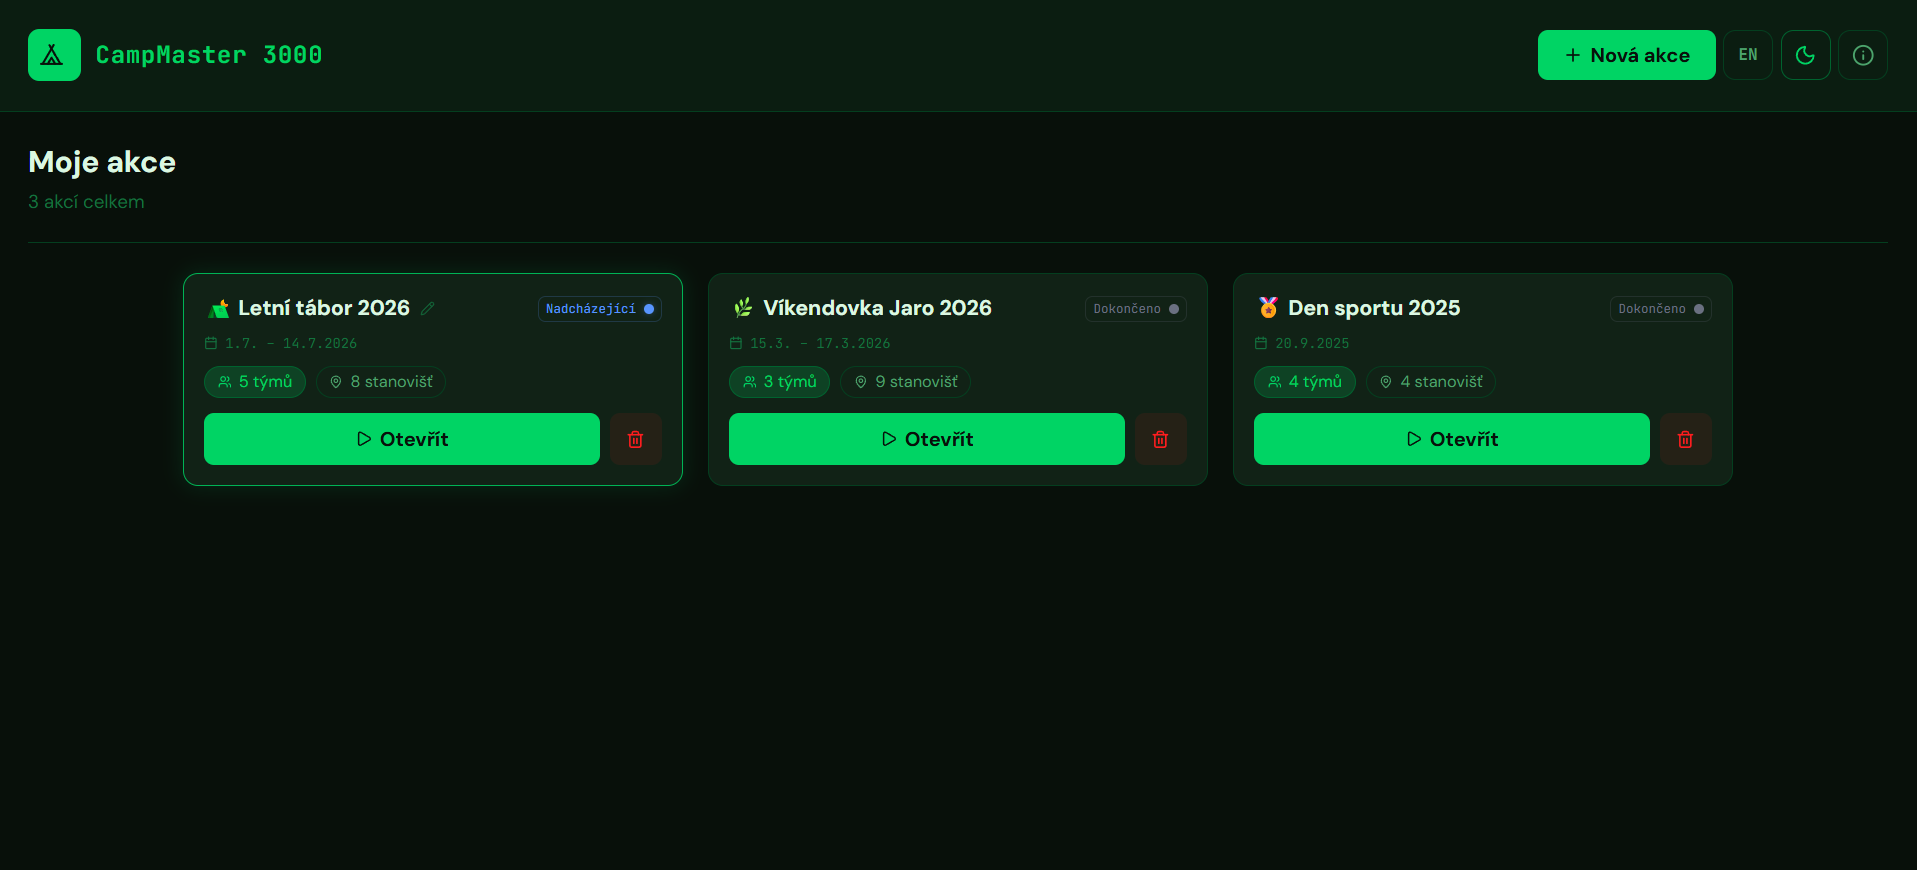
\includegraphics[width=\textheight,keepaspectratio]{img/screenshot-home.png}%
  }{%
    \fbox{\parbox[c][10cm][c]{0.97\textheight}{\centering\color{gray}\texttt{img/screenshot-home.png}}}%
  }
  \caption{Domovská obrazovka — přehled karet akcí s~hover efektem tužky pro přejmenování}
  \label{fig:home}
\end{sidewaysfigure}

\begin{sidewaysfigure}
  \centering
  \IfFileExists{img/screenshot-wizard.png}{%
    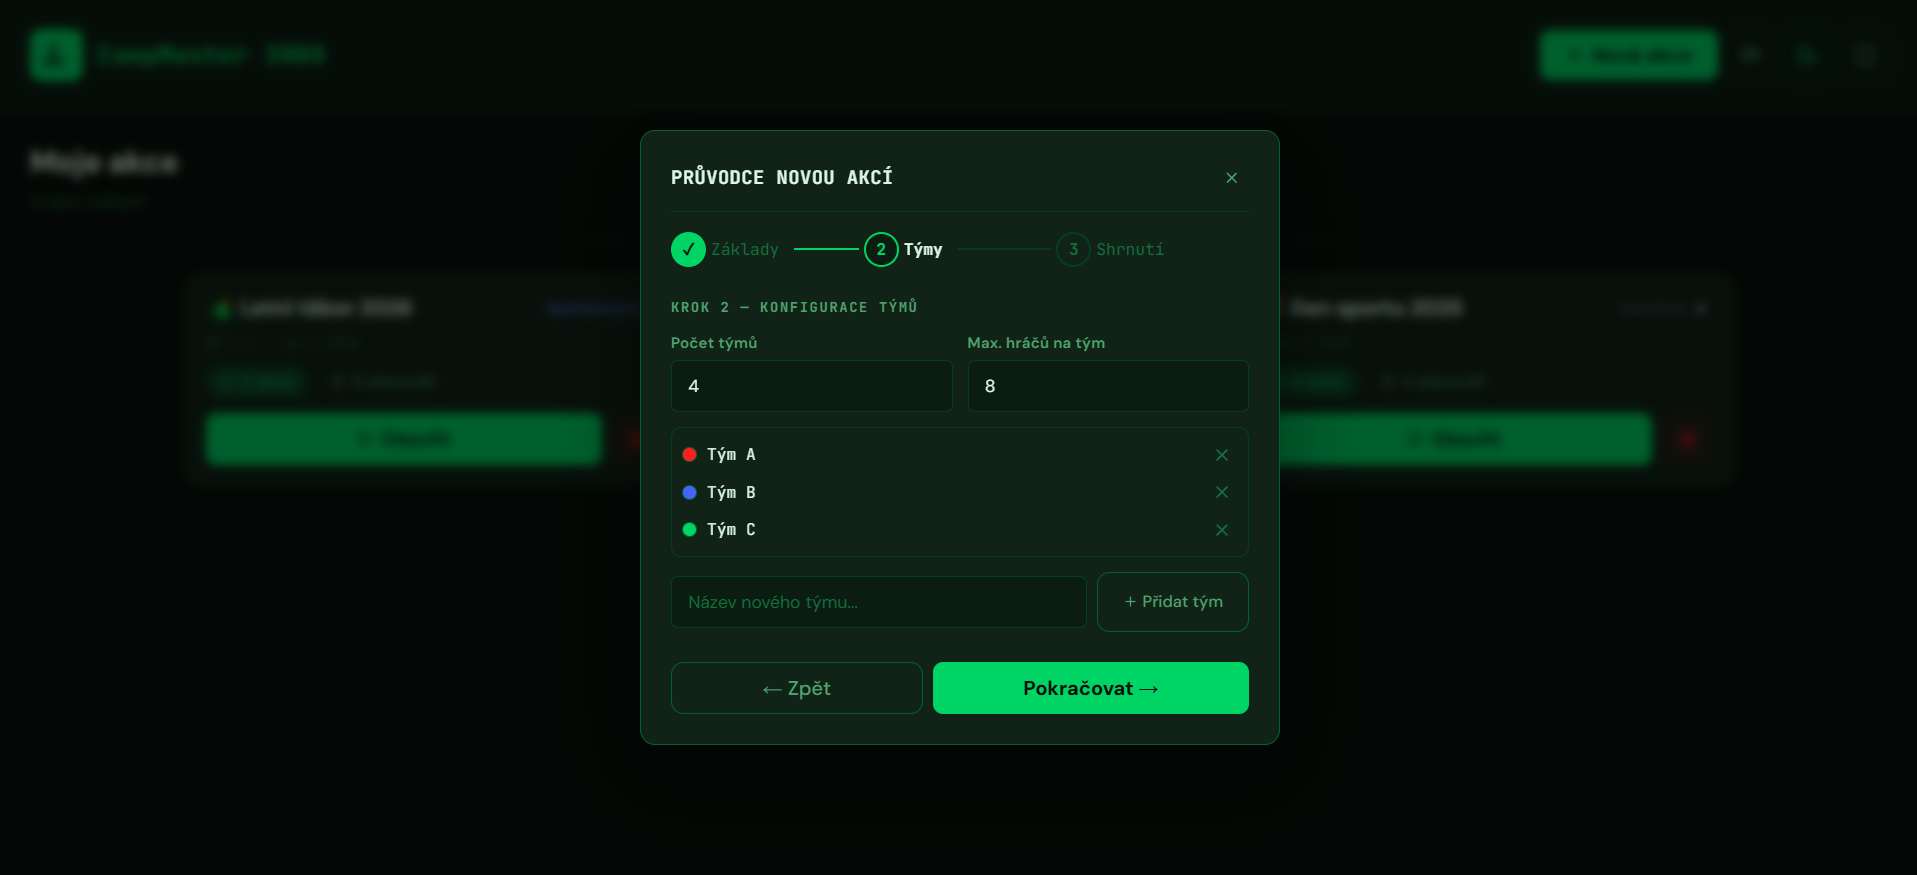
\includegraphics[width=\textheight,keepaspectratio]{img/screenshot-wizard.png}%
  }{%
    \fbox{\parbox[c][10cm][c]{0.97\textheight}{\centering\color{gray}\texttt{img/screenshot-wizard.png}}}%
  }
  \caption{Průvodce novou akcí — krok 2 (konfigurace týmů)}
  \label{fig:wizard}
\end{sidewaysfigure}

\begin{sidewaysfigure}
  \centering
  \IfFileExists{img/screenshot-editor.png}{%
    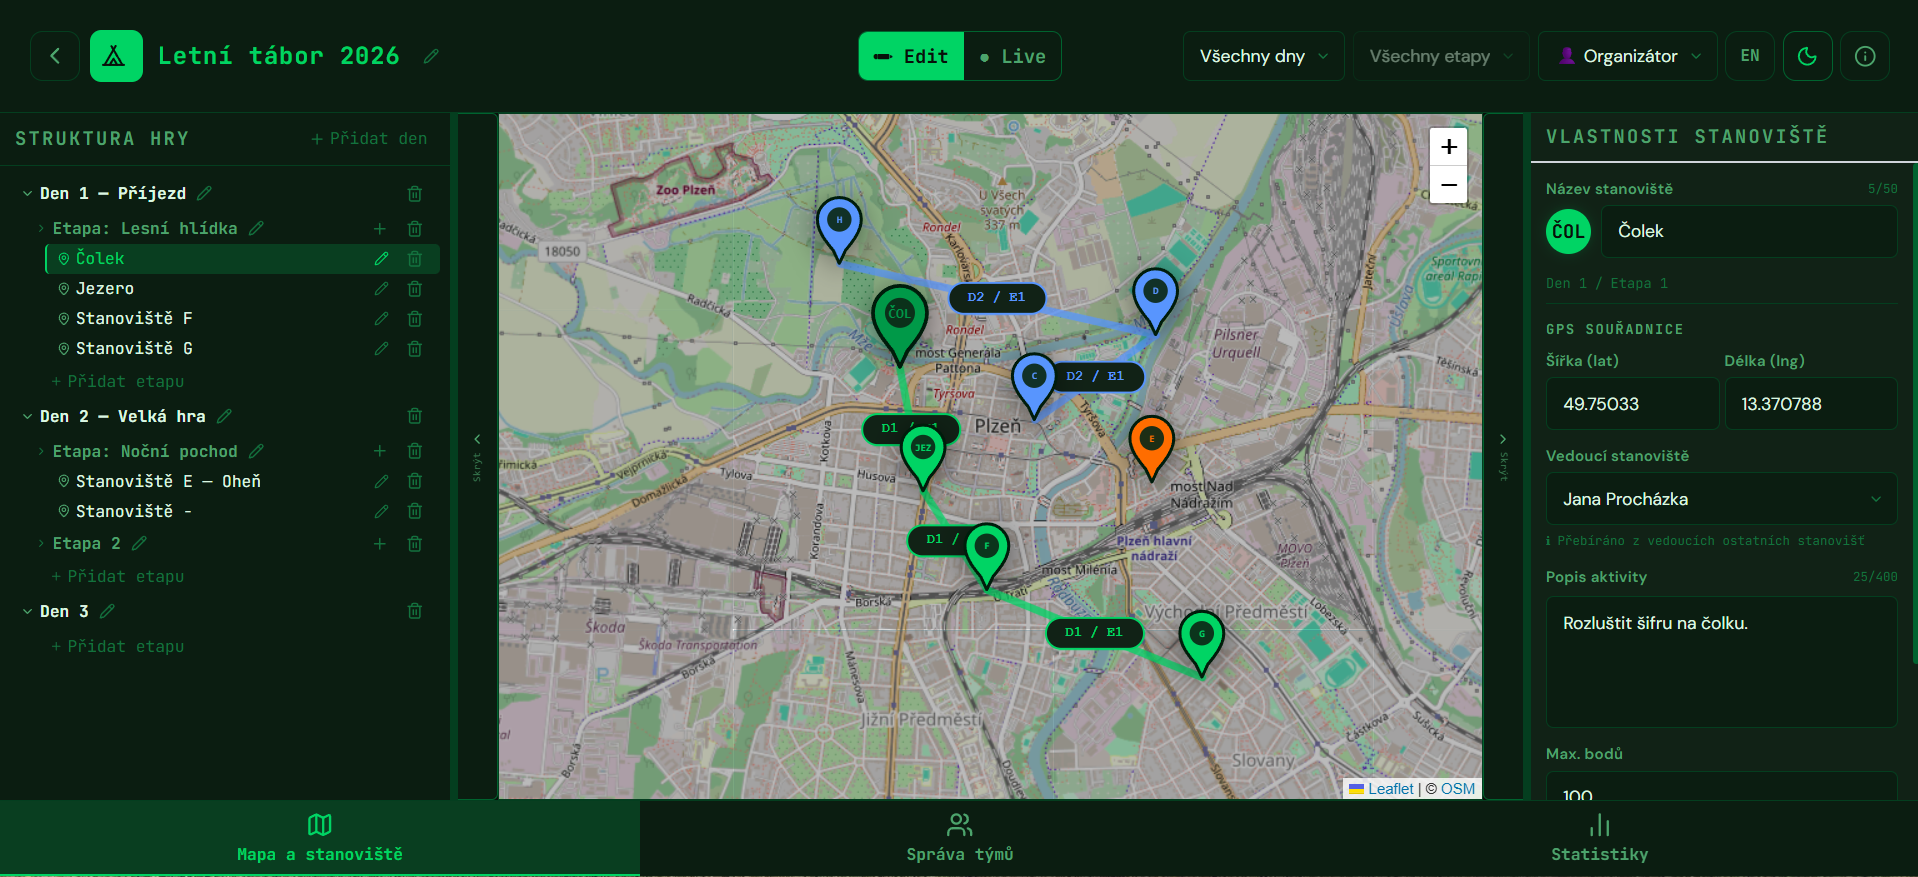
\includegraphics[width=\textheight,keepaspectratio]{img/screenshot-editor.png}%
  }{%
    \fbox{\parbox[c][10cm][c]{0.97\textheight}{\centering\color{gray}\texttt{img/screenshot-editor.png}}}%
  }
  \caption{Editor — tři resizovatelné panely: GameTree (vlevo), mapa Leaflet (střed), PropertiesPanel (vpravo)}
  \label{fig:editor}
\end{sidewaysfigure}

\begin{sidewaysfigure}
  \centering
  \IfFileExists{img/screenshot-live-stations.png}{%
    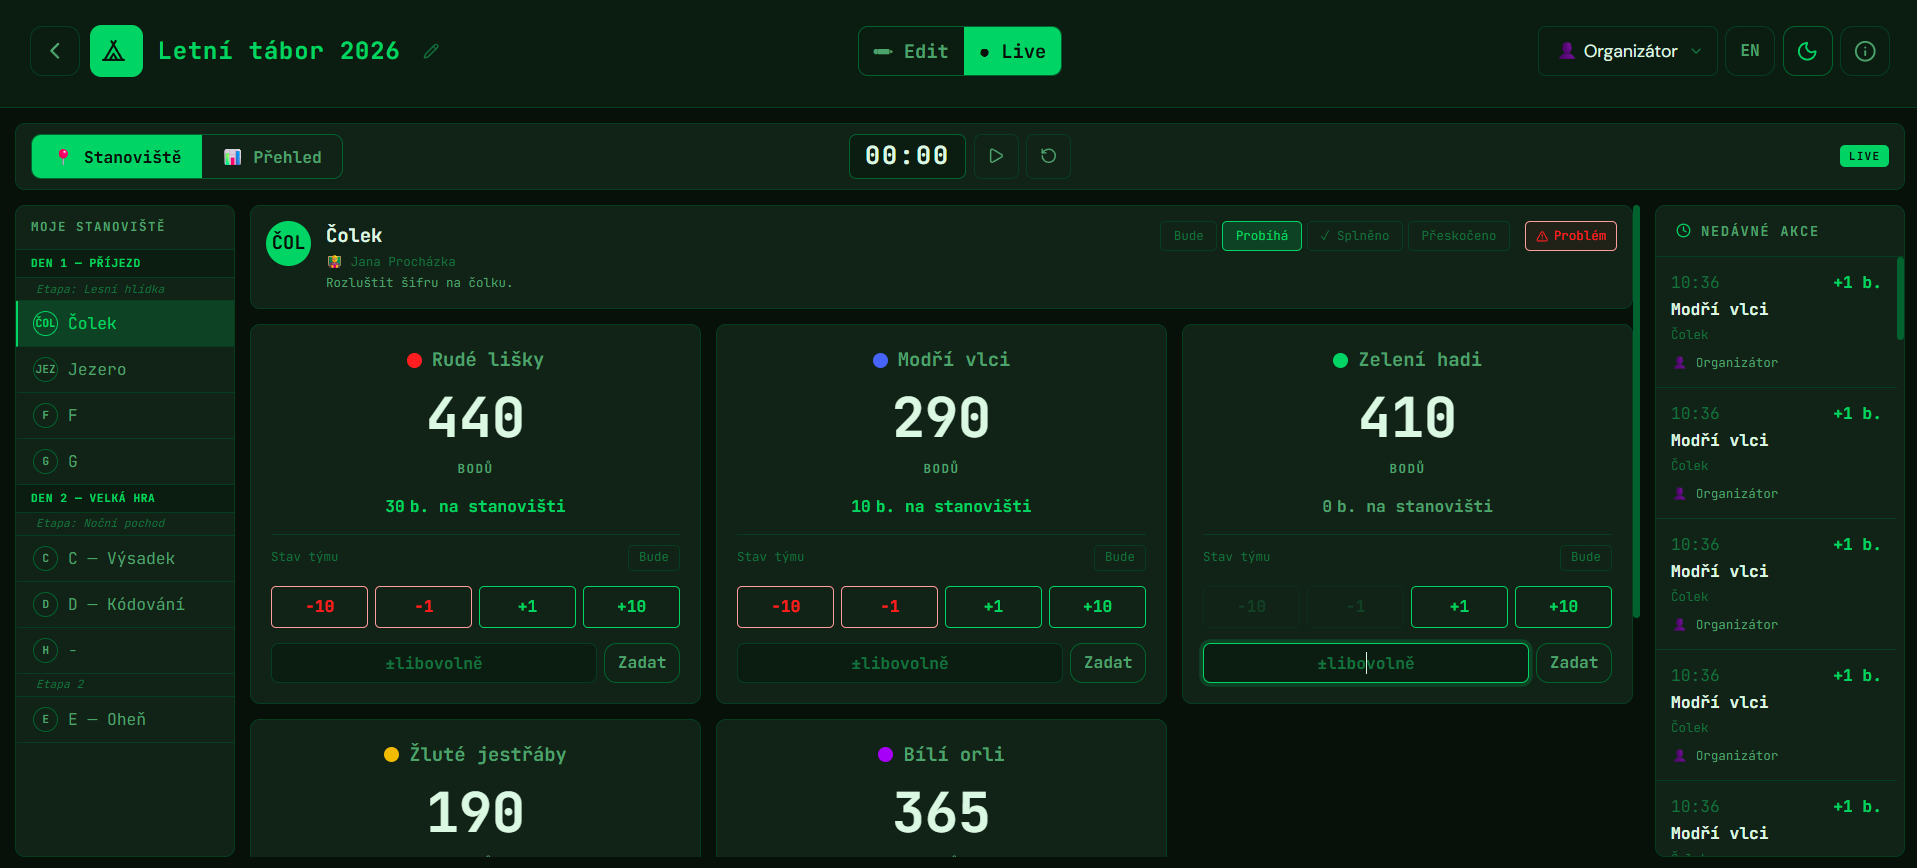
\includegraphics[width=\textheight,keepaspectratio]{img/screenshot-live-stations.png}%
  }{%
    \fbox{\parbox[c][10cm][c]{0.97\textheight}{\centering\color{gray}\texttt{img/screenshot-live-stations.png}}}%
  }
  \caption{Live mód — záložka Stanoviště: karty týmů s~bodovým vstupem a~per-stanoviště skóre}
  \label{fig:live-stations}
\end{sidewaysfigure}

\begin{sidewaysfigure}
  \centering
  \IfFileExists{img/screenshot-live-overview.png}{%
    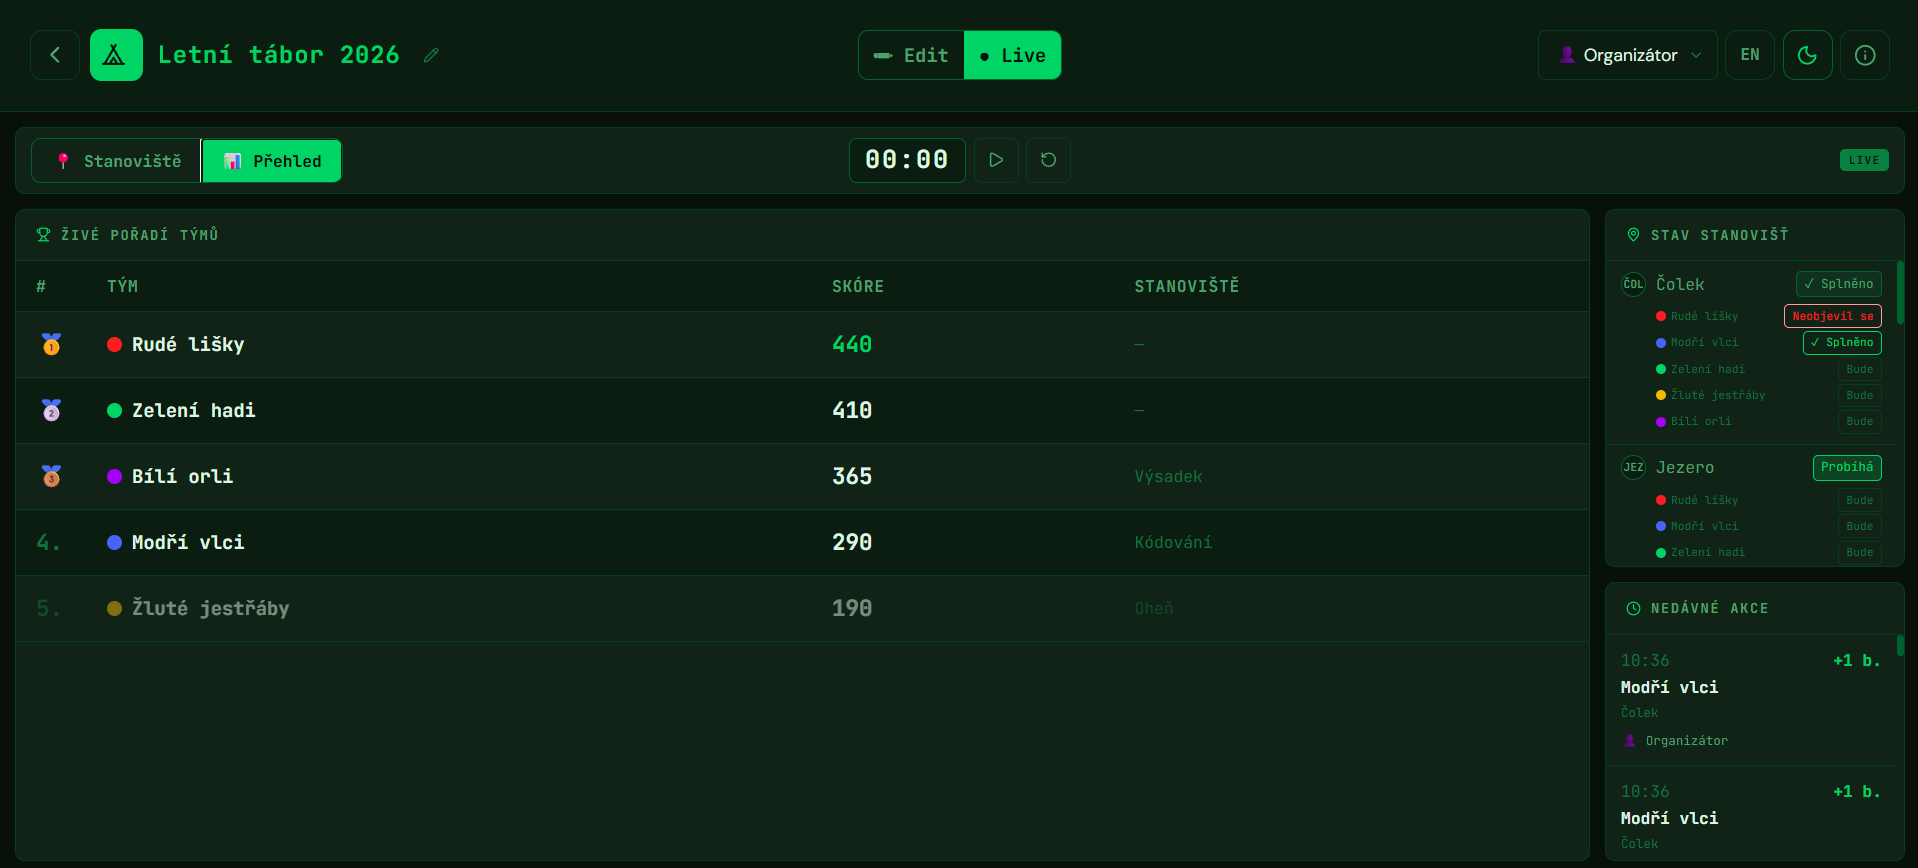
\includegraphics[width=\textheight,keepaspectratio]{img/screenshot-live-overview.png}%
  }{%
    \fbox{\parbox[c][10cm][c]{0.97\textheight}{\centering\color{gray}\texttt{img/screenshot-live-overview.png}}}%
  }
  \caption{Live mód — záložka Přehled: živý žebříček a~panel stavu stanovišť}
  \label{fig:live-overview}
\end{sidewaysfigure}

\end{document}
